\documentclass[tikz,border=2pt]{standalone}
\usepackage{tikz}
\usetikzlibrary{arrows,calc}

\begin{document}

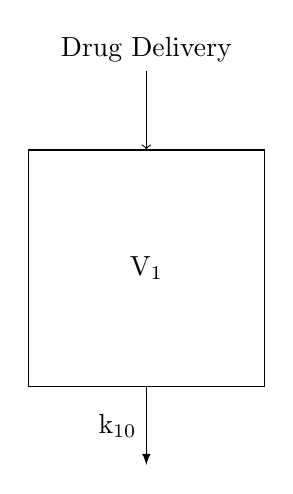
\begin{tikzpicture}
% boxes
\node[draw,minimum width=3cm, minimum height=3cm] (a) at (0,0) {V\textsubscript{1}};


% compute a point in the middle between E and NE or W and NW, then draw a line between these two

\draw[->, black] (0,2.5) node[above, black]{Drug Delivery} --   (a.north);

\draw[->, latex-] (0,-2.5) --  node[left, black]{k\textsubscript{10}} (a.south);


\end{tikzpicture}

\end{document}